\documentclass[11pt]{article}
\usepackage[margin=1in]{geometry}
\usepackage{amsmath,amssymb,booktabs,url,xcolor}
\usepackage[hidelinks]{hyperref}
\usepackage{graphicx}
\emergencystretch=1.5em

\title{Staged Upgrades of Two Learned Populations: Recovering Part of a Learned Fleet's Benefit When the Signals It Relies On Are Upgraded\\[4pt]
\large DRAFT (05/10/2026)}
\date{}

\begin{document}
\maketitle

\begin{abstract}
Learned traffic signals and learned connected-vehicle fleets are owned by different parties and upgraded on different schedules. We study
what happens to a learned eco-driving fleet when the signals it relies on are upgraded to a learned adaptive controller, and how to repair
the loss without retraining either population. In SUMO on a 16-signal grid, a PPO fleet that saves fuel against its base driver under
fixed-time signals loses that benefit once the signals become learned: withdrawing the timing returns it to its base driver, and
forecasting the learned signal's timing costs the fleet's own vehicles time. Light-side repairs (commitments, gates, predictable splits)
cost more than they recover. A publication / shadow comparison, an input intervention and an open-loop replay support a closed-loop
account: once timing is published, the fleet's slower approach changes the demand that the halting-based signal observes, the signal holds
its greens longer, and the forecast's own target shifts. We propose a two-sided interface (TSI) between the frozen policies: for the fleet,
a state-conditioned forecast with exact answers where the timing is already determined; for the signal, a speed-binned demand count in front
of its inputs. Both are calibrated per deployed signal controller on training and tuning traffic. In the second registered confirmation
(the first, with one global adapter, failed on the fleet's time loss), on the same five signal checkpoints and four frozen fleets as the
first attempt with fresh traffic (family-wise bound 0.075), TSI reduces the fleet's fuel by $3.85\%$ (95\% CI $[3.26, 4.43]$), city time
loss by $0.55$\,s/veh and human time loss by $0.89$\,s/veh, with the fleet's time loss non-inferior at a $+0.5$\,s/veh margin (one-sided
$\alpha=0.025$). The same configuration met every limit again on a third fresh traffic panel ($-3.70\%$ fuel). Against the repository's
fleet-retraining recipe on the same panels, no fuel difference was detected; the interval contains 0 and this is not an equivalence test,
so equality with retraining is not shown, while TSI's time losses were lower. A DC-Ada-style affine input adaptation at matched rollout
budget returned the identity transform and missed the fleet-time limit; it is not a faithful reproduction of the published method, and we
claim no win over it or over any published method. On a second network with multi-green learned signals and a rule fleet the method failed
three registered attempts. The evidence supports a useful method that meets the registered joint objective where several internal
comparators do not, in one setting; it is not a general or state-of-the-art result.
\end{abstract}

\section{Introduction}
Connected vehicles can save fuel by adapting their approach speed to the signal phase and timing (SPaT) that intersections broadcast:
green-light optimal speed advisory (GLOSA) and predictive cruise control avoid stops when the time to the next green is known
\cite{katsaros2011,asadi2011}. Signals, in turn, are moving from fixed programs to learned adaptive controllers trained with reinforcement
learning on detector data \cite{wei2018,wei2019,ault2021}. The two technologies are owned by different parties: the city or its supplier
upgrades the signals, a manufacturer or fleet operator updates the vehicles' controllers, and the two release schedules are independent.

This creates a compatibility problem between two learned populations. A fleet trained against static programs uses SPaT as if it were a
plan. Once the signals are upgraded to a learned controller, the timing is no longer a plan: the signal decides every few seconds from what
it observes. The fleet's information channel then either disappears (the signal publishes nothing it can guarantee) or becomes a forecast,
and a forecast of an adaptive signal is known to be hard to make reliable \cite{bodenheimer2014,genser2024,eteifa2025}. The question is
related to the compatibility of model updates with their users \cite{bansal2019} and to coordination with unfamiliar partners
\cite{stone2010,hu2020}. Here the two partners are frozen learned policies coupled through a physical traffic system and an information
channel, and the only levers are the interfaces between them.

We ask whether a deployed learned fleet can keep or recover its benefit when the learned signals it relies on are upgraded,
\emph{without retraining either population}. We build a staged-upgrade benchmark in SUMO \cite{lopez2018} with registered gates and
fresh-traffic confirmations and find four things.
\begin{enumerate}\setlength\itemsep{1pt}
\item \emph{The loss is real.} A learned fleet that saves fuel under fixed-time signals loses its benefit after the upgrade. With the
timing withdrawn it falls back exactly to its base driver; with the old program still derived as SPaT it is harmed.
\item \emph{The obvious repairs fail.} A forecast of the learned signal costs the fleet's own vehicles time. Making the signal commit to
its timing, gating the forecast, or replacing the signal by a predictable split controller costs more than the fleet recovers.
\item \emph{The cause is a closed loop.} Publishing a forecast changes the fleet's approach, which changes what the halting-based signal
observes, which changes the signal's timing and therefore the forecast's own target. This is a traffic-signal instance of the consistency
problem of anticipatory guidance \cite{bottom2000} and of performative prediction \cite{perdomo2020,narang2023}.
\item \emph{Two interfaces together repair it in one setting.} A two-sided interface (TSI) calibrates a state-conditioned forecast for the
fleet and a speed-binned demand count for the signal, per deployed signal controller, with neither policy retrained.
\end{enumerate}

\paragraph{Contributions.}
(i) A staged-upgrade benchmark with two learned populations (learned keep-or-switch signals; PPO and search-fitted eco-driving fleets, with
a fixed rule fleet as a non-learned receiver), registered gates, and fresh-data confirmations (M1--M2).
(ii) A negative map of light-side and information-only repairs, each tested against the no-SPaT fallback. In our measurement,
per-decision counterfactual credit was below the simulator's chaotic noise floor (signal-to-noise about 0.2).
(iii) A closed-loop diagnosis from three diagnostics (publication / shadow, an input intervention, an open-loop replay), with no single
mediator isolated. Once timing is published, the halting-based learned signal sees less of the fleet's demand and holds its greens longer,
and the forecast's own target shifts (a performative feedback). On a fixed schedule, exact timing costs the fleet no time.
(iv) The two-sided interface TSI, with a calibration procedure whose cost is stated. It was confirmed in a second registered attempt on the
same five light and four fleet checkpoints as the failed first attempt (whose per-light results motivated per-light calibration; fresh
traffic; family-wise bound 0.075) and met the limits again on a third fresh traffic panel. It comes with component ablations, same-panel
comparisons with fleet retraining, and scope tests across receiver classes, penetration and demand.
(v) Additional registered comparators and failures, reported in full: a DC-Ada-style input adaptation, two retraining variants, a learned
predictable-signal reference, a learned-to-learned signal swap, and three failed attempts on a second network.

\paragraph{Claim boundary.} The evidence supports a useful method that meets the registered joint objective (fuel saving with time-loss
non-inferiority) where several internal comparators do not, in one network. It does not
show equality with retraining on fuel: no fuel difference was detected, which is not an equivalence test. It does not show a win over any
published method under the same rights and budget, and it is not a state-of-the-art claim. The confirmations reuse policy checkpoints
across attempts, so they are fresh-traffic, not fresh-policy, replications. The method failed on the second network.

\paragraph{Outline.} Section~\ref{sec:related} reviews related work. Section~\ref{sec:setting} defines the setting, rights and endpoints;
Section~\ref{sec:method} gives TSI; Section~\ref{sec:setup} the experimental setup; Section~\ref{sec:results} the results;
Section~\ref{sec:discussion} what they support; and Sections~\ref{sec:limits}--\ref{sec:repro} limitations and reproducibility.

\section{Related work}\label{sec:related}
\paragraph{Eco-driving with signal information.} GLOSA advises a speed that reaches the stop line at green
\cite{katsaros2011}. Predictive cruise control optimizes the velocity trajectory over upcoming signal states \cite{asadi2011}. Both assume
that the time to green is known. For adaptive signals the advisory needs a prediction of the signal's own decisions, and its quality limits
the benefit \cite{bodenheimer2014}. Our fleets are of this kind: a GLOSA rule with lane-aware release, a search-fitted variant, and a PPO
residual on the rule.
\paragraph{Learned signal control.} Deep RL controllers learn phase decisions from queue or pressure observations \cite{wei2018,wei2019}.
Pressure-based designs are motivated by max-pressure control, which is throughput-optimal under a queueing model \cite{varaiya2013}, and
benchmark suites compare controllers in SUMO \cite{ault2021}. Our learned signal is a deliberately simple keep-or-switch DQN on halting and
vehicle counts. It stands for signals whose inputs count stopped vehicles; we make no claim about other input designs, and we do not claim
it is a state-of-the-art signal controller.
\paragraph{SPaT prediction for adaptive and actuated signals.} Supervised time-to-green models predict actuated signals from detector and
signal data \cite{genser2024}. Deep ensembles attach a confidence level \cite{eteifa2025}. Prediction methods for adaptive lights trade
accuracy against horizon \cite{bodenheimer2014}. Our forecaster belongs to this line and is not new; it meets the joint objective only in
combination with the light-side adapter.
\paragraph{Joint signal--vehicle learning and predictable signals.} CoTV controls signals and the nearest connected vehicle on each
approach with multi-agent deep RL \cite{guo2023}. HONEST-CAV optimizes network signals and vehicle trajectories hierarchically with
value-decomposition MARL \cite{zhang2026}. DHCP plans a predictable cycle with hierarchical deep RL \cite{gu2025}. These methods train or
co-design both sides, or redesign the signal. Our setting has fewer rights: both populations are frozen and upgraded on separate schedules,
and only the interfaces may change. Our learned predictable-signal reference (Section~\ref{sec:w6}) is structural only; it is not a
reproduction of DHCP.
\paragraph{Compatibility of updates and partners.} An update that improves an AI system can hurt the team that relies on it
\cite{bansal2019}. Ad hoc teamwork and zero-shot coordination ask for agents that work with unfamiliar partners
\cite{stone2010,hu2020}. Our setting is a two-population, physically coupled instance: the partner changes by an upgrade, and the repair
must act through the information and sensing interfaces rather than through either policy.
\paragraph{Observation adapters for frozen policies.} DC-Ada adapts per-robot observation transforms of a frozen shared policy by
reward-only random search \cite{alqithami2026}. Adaptive modular world models separate a site-specific observation adapter from a shared
dynamics model for traffic-signal transfer \cite{huang2026}. Our adapter is a two-parameter physical count transform calibrated against a
partner-induced shift rather than a sensing-pipeline change. A DC-Ada-style affine adaptation at matched budget is among our comparators
(Section~\ref{sec:w6}), with its differences from the published method stated.
\paragraph{Performative feedback.} When published forecasts change the outcome they forecast, a forecast is useful only if it is consistent
with the reaction it causes. This is the consistency requirement of anticipatory route guidance \cite{bottom2000}, and it is studied as
performative prediction \cite{perdomo2020} and as optimization with decision-dependent distributions \cite{drusvyatskiy2023}. With several
decision makers it becomes a multiplayer game \cite{narang2023}. We identify a traffic-signal instance and show, on development traffic,
that a light-side input change reduces the measured sensitivity. The complementarity of the two interfaces is consistent with a small-gain
reading of the loop forecast $\to$ fleet $\to$ light $\to$ target \cite{jiang1994,dashkovskiy2007}. This is motivation, not a theorem
about the learned light: our policies are frozen and non-convex, and none of these results' hypotheses is verified here.
\paragraph{Position.} No published method was reproduced under the same rights and budget. We therefore make no state-of-the-art or
``first'' claim. Forecaster plus adapter is not by itself a novel combination; the contribution is the closed-loop diagnosis and the
confirmed two-sided calibration procedure in this setting.

\section{Problem setting}\label{sec:setting}
\paragraph{Populations and interfaces.} A network has signal controllers $i\in\mathcal I$ and vehicles $v$. A share $\rho$ of the vehicles
are fleet agents: membership is fixed per vehicle id by a stable hash, so it is identical across all arms. Two frozen policies act:
\begin{itemize}\setlength\itemsep{0pt}
\item the signal policy $\pi_L$, shared by every controller, which maps its input $o_{i,t}$ to keep or switch;
\item the fleet policy $\pi_F$, which maps an agent's state and the SPaT answer $s=(\mathit{ttg},\mathit{ttr},\mathit{valid})$ to a speed
command.
\end{itemize}
They interact through two interfaces:
\begin{equation}
o_{i,t} = g\big(z_{i,t}\big), \qquad s_{v,t} = P\big(x_{i,t}, \ell_v\big),
\end{equation}
where $z_{i,t}$ is the raw lane sensing at controller $i$ (counts and speeds), $g$ is the signal's input map (the identity on halting
counts for the deployed controller), $x_{i,t}$ is the controller's state (phase, time in phase, sensing), $\ell_v$ the link the agent is
approaching, and $P$ the SPaT provider. When $P$ returns $\mathit{valid}=0$, the fleet releases control to its base driver.
\paragraph{Rights.} After the upgrade, the weights of $\pi_L$ and $\pi_F$ are frozen. Only $g$ and $P$ may change. They may be fitted or
tuned from simulated episodes of the deployed controller with a development fleet on training and tuning traffic, never on confirmation
traffic or with confirmation fleets. Retraining $\pi_F$ (more rights) is a reference, not a competitor under the same rights.
\paragraph{Outcomes and endpoints.} For an episode with traffic seed $s$, light checkpoint $l$ and fleet checkpoint $f$, let $F_A$ be the
agents' total fuel (SUMO emission model), and let $\mathrm{TL}$, $\mathrm{TL}_A$, $\mathrm{TL}_H$ be the mean time loss of all vehicles,
of agents and of human-driven vehicles (s/veh; trips unfinished at the end are counted with their time loss so far). The reference arm R
is the upgraded signal with no SPaT ($P\equiv$ unavailable), under which the fleet drives exactly as its base driver $\sigma^*$. For an arm
X the cell-level effects are
\begin{equation}
\Delta F[l,f,s] = 100\Big(\frac{F_A^{X}}{F_A^{R}}-1\Big), \qquad \Delta\mathrm{TL}_\bullet[l,f,s]=\mathrm{TL}_\bullet^{X}-\mathrm{TL}_\bullet^{R},
\end{equation}
with both arms run on the same cell.
\paragraph{Statistics.} Effects are averaged over the crossed panel $D\in\mathbb R^{L\times F\times S}$. Uncertainty comes from a crossed
bootstrap: draw $l^*$, $f^*$, $s^*$ independently with replacement from the light, fleet and traffic indices; set
$\hat\theta^*_b=\overline{D[l^*,f^*,s^*]}$; repeat $B=2000$ times. Two-sided 95\% intervals are the 2.5\% and 97.5\% quantiles, and the
one-sided upper bound at level $\alpha$ is $U_{1-\alpha}=\mathrm{quantile}_{1-\alpha}(\hat\theta^*)$. When light sets differ between
arms, light indices are resampled separately per arm, with fleets and traffic shared.
\paragraph{Feasibility (registered M3 limits).} An arm meets the limits against R iff
\begin{equation}
U_{1-\alpha}(\Delta F)<0,\quad U_{1-\alpha}(\Delta\mathrm{TL}),\,U_{1-\alpha}(\Delta\mathrm{TL}_A),\,U_{1-\alpha}(\Delta\mathrm{TL}_H)<\delta=0.5\,\mathrm{s/veh},
\end{equation}
and its teleports per run do not exceed R's by more than 0.1, with unfinished trips not above R's.
\begin{itemize}\setlength\itemsep{0pt}
\item $\alpha=0.05$ for a first registered attempt and for descriptive scope tests.
\item $\alpha=0.025$ for a second attempt and $0.0125$ for a third; the family-wise bound over a chain of attempts is the sum (Bonferroni).
\item A failed limit is reported as ``not shown''; it is not read as evidence of harm.
\end{itemize}

\section{Method: a two-sided interface (TSI)}\label{sec:method}
TSI changes the two interfaces $P$ and $g$ and nothing else (Figure~\ref{fig:schematic}).
\begin{figure}[t]\centering\includegraphics[width=0.95\linewidth]{figs_two_pop/p1_schematic.pdf}
\caption{The setting and the two interfaces TSI changes (blue). Both learned policies are frozen. The orange path is the closed loop
diagnosed in Section~\ref{sec:diag}.}\label{fig:schematic}\end{figure}
\subsection{Fleet side: a hybrid provider}
Let $c_{i}(t)$ be controller $i$'s current phase, $\mathcal G_i$ its green phases, and $\mathrm{serve}(\ell)\subseteq\mathcal G_i$ the
greens serving link $\ell$.
\begin{itemize}\setlength\itemsep{0pt}
\item \emph{Determined case.} During a yellow, the next green is fixed by the program. If that green serves $\ell$, the provider answers
with the table forecast's yellow branch, $\mathit{ttg}=(Y-\tau)+o$, which is exact there (C-113). Here $Y=3$\,s is the yellow length,
$\tau$ the time in the yellow, and $o=1$\,s the simulator's one-step observation offset.
\item \emph{Every other query} is answered by a state-conditioned forecaster at its median.
\end{itemize}
Together,
\begin{equation}
P_{\mathrm{hyb}}(x_{i,t},\ell)=\begin{cases}\text{table answer (exact)} & c_i(t)\ \text{yellow and next green}\in\mathrm{serve}(\ell),\\
\big(\hat y_{0.5}(x_{i,t},k),\ \mathit{valid}=1\big) & \text{otherwise,}\end{cases}
\end{equation}
where $k$ is the event kind: the end of the current green (time to red) or the next onset of the other green (time to green).
\paragraph{Forecaster.} The features $\phi(x_{i,t},k)$ are:
\begin{itemize}\setlength\itemsep{0pt}
\item the phase one-hot and the time in phase;
\item the event kind;
\item halting and vehicle counts on the lanes of the current and the target green;
\item the recent green-duration history;
\item the light one-hot.
\end{itemize}
The target $y$ is the realized time to the event, and censored rows are dropped. A multilayer perceptron $f_\theta$ (two hidden layers of
64 units) outputs two monotone quantiles $q\in\{0.1,0.5\}$ and is fitted by minimizing the query-weighted pinball loss
\begin{equation}
\mathcal L(\theta)=\sum_j w_j\sum_{q\in\{0.1,0.5\}}\rho_q\big(y_j-f_\theta(\phi_j)_q\big),\qquad \rho_q(u)=\max\{qu,(q-1)u\},\qquad w_j=0.25+Q_j,
\end{equation}
where $Q_j$ is the number of fleet queries at that light-second, so the fit is weighted toward where the fleet asks.
\begin{itemize}\setlength\itemsep{0pt}
\item \emph{Data:} eight TRAIN episodes per deployed light (seeds 0--5 for fitting, 6--7 for validation), with the development fleet
querying the age-conditioned table forecast (c2, 0.1 quantile).
\item \emph{Optimizer:} Adam with step size $10^{-3}$, batches of 8192, at most 40 epochs, keeping the epoch with the best validation loss.
\item \emph{Served quantile:} the median, $\hat y_{0.5}=f_\theta(\phi)_{0.5}$.
\end{itemize}
\subsection{Light side: a speed-binned demand count}
The deployed signal's inputs include, for each of its two greens $g$, the halting count on the served lanes divided by 10. TSI replaces this
count by
\begin{equation}
q_g=\sum_{v\in\mathrm{lanes}(g)}\Big(\mathbb 1\{u_v<0.1\}+A\,\mathbb 1\{0.1\le u_v<2\}+B\,\mathbb 1\{2\le u_v<5\}\Big),\qquad o_g=q_g/10,
\end{equation}
where $u_v$ is a vehicle's speed (m/s). All other inputs, the decision rule and the weights are unchanged, and $A=B=0$ recovers the deployed
signal exactly. The intent is to count the slow eco-approaching vehicles that the 0.1\,m/s halting threshold no longer sees. The adapter
does more than restore demand perception, so no single mediator is claimed.
\subsection{Calibration per deployed signal controller}
For each deployed controller (light checkpoint):
\begin{enumerate}\setlength\itemsep{0pt}
\item \emph{Forecaster.} Log eight TRAIN episodes with the development fleet and fit $f_\theta$ as above.
\item \emph{Adapter grid.} Run R and every $(A,B)$ in
\[\mathcal C=\{(1,0),(1.5,0),(2,0),(1,0.25),(1.5,0.25),(2,0.25),(1,0.5),(1.5,0.5),(2,0.5),(3,0.5)\},\]
with the hybrid provider on, on four TUNE episodes. Let $m_\bullet(A,B)$ be the mean differences against R on those episodes.
\item \emph{Selection} (registered):
\begin{gather}
\mathcal S=\{(A,B)\in\mathcal C: m_{\mathrm{TL}_A}\le-0.25,\ m_{\mathrm{TL}}\le0,\ m_{\mathrm{TL}_H}\le0\},\\
(A^*,B^*)=\begin{cases}\arg\min_{\mathcal S} m_{F} & \mathcal S\neq\emptyset,\\ \arg\min_{\mathcal C} m_{\mathrm{TL}_A} & \text{otherwise,}\end{cases}
\end{gather}
with ties broken by the smaller $A+B$.
\end{enumerate}
The stricter $-0.25$\,s/veh threshold on the agents' time point leaves room for tuning-to-confirmation shrinkage.
\paragraph{Calibration cost (per deployed light controller).}
\begin{itemize}\setlength\itemsep{0pt}
\item \emph{Forecaster:} 8 TRAIN episodes with the fleet using the age-conditioned table forecast (feature log), plus one fit of the
64--64 MLP (CPU, about 30\,s, 40 epochs).
\item \emph{Adapter:} 10 grid points and R on 4 TUNE episodes each, 44 episodes. In total, 52 simulated episodes per light.
\item \emph{No policy-gradient step} for either population.
\item \emph{Sensors:} the halting and vehicle counts already used by the signal, plus vehicle speeds on the served lanes (three speed bins).
\item \emph{Inference:} one MLP pass per light and second when the fleet queries; the table answer in the determined case.
\end{itemize}
\paragraph{Multi-green signals.} For a signal with $K\in\{2,3\}$ greens (Section~\ref{sec:m4}), the features are taken relative to the
current green: the number of greens to pass before the target (one-hot), and halting / vehicle counts at relative cycle positions 0, 1 and
2. The adapter acts on the current and the next green's inputs.

\section{Experimental setup}\label{sec:setup}
\paragraph{Simulator.} SUMO 1.27.1 \cite{lopez2018} through its Python interface: 1\,s steps, teleport after 300\,s of blocking, the
emission device on every vehicle (fuel from SUMO's default emission model), departures over 3600\,s. Trip records include unfinished trips.
Runs are deterministic given the seed (PYTHONHASHSEED = 0, OMP\_NUM\_THREADS = 1; bit-identical repeats checked, C-27).
\paragraph{Networks and demand.}
\begin{itemize}\setlength\itemsep{0pt}
\item \emph{grid4:} a $4\times4$ grid with 16 signals. Each signal has two greens and two fixed 3-s yellows, with permissive left turns.
\item \emph{spider} (second network): built with SUMO's \texttt{netgenerate}; 18 signals, 12 with two greens and 6 with three.
\item \emph{Demand:} generated by \texttt{randomTrips} with one departure every 2.0\,s (1\,800\,veh/h), fringe factor 10 and minimum trip
distance 300\,m; the demand-shift test uses 1.6\,s (+25\%). Every evaluation panel was generated only after a check that its seeds did not
already exist (Table~\ref{tab:panels}).
\end{itemize}
\paragraph{Learned signal (RL-H).} A keep-or-switch DQN decides every 5\,s, with a minimum green of 5\,s; a switch starts the fixed yellow.
\begin{itemize}\setlength\itemsep{0pt}
\item \emph{Input:} $[h_1/10,h_2/10,n_1/20,n_2/20,\mathbb 1\{\text{green }1\},\mathbb 1\{\text{green }2\},\tau/60]$, with halting $h$ and
vehicle counts $n$ on the lanes of the two greens and $\tau$ the time in phase.
\item \emph{Reward:} $-(\text{halting on incoming lanes})/10$.
\item \emph{Training:} double DQN with two 64-unit ReLU layers, $\gamma=0.9$, Adam ($10^{-3}$), a replay of $2\times10^5$, batches of 256,
200 updates per episode, $\varepsilon$ from 1 to 0.05 over the first 60\% of 120 episodes, on TRAIN seeds 0--7 with SUMO cars.
\item \emph{Behaviour:} under RL-H the mean green is about 15\,s, against 42\,s under the fixed-time program (C-100).
\item \emph{Seeds:} development k0 / k1; confirmation t4--t8.
\item \emph{Spider:} a keep-or-advance DQN over its $K$ greens with halting-based inputs and reward, 120 episodes (C-76).
\end{itemize}
\paragraph{Fleets.} Agents are 50\% of vehicles. Their base driver is SUMO's Krauss model with imperfection $\sigma^*=0.3$, chosen on SELECT
100--104 (M1).
\begin{itemize}\setlength\itemsep{0pt}
\item \emph{Rule fleet GLOSA-L$\circ\sigma^*$ (R8).} Within 200\,m of a signal whose movement is not green, with valid SPaT, it commands
$v_{\mathrm{rule}}=\min(v_{\mathrm{allowed}},d/\mathit{ttg})$. It releases control when the current lane does not continue on the route,
which removes the lane-change deadlocks of speed commands (C-45, C-46).
\item \emph{Search-fitted fleet R9.} Four parameters of the rule, including the release distance, fitted by derivative-free search on
training traffic (C-54).
\item \emph{PPO fleet R10.} A residual on the rule, acting only where the rule commands:
\[\mathrm{cmd}=\mathrm{clip}\big(v_{\mathrm{rule}}+3\tanh u,\ 0,\ v_{\mathrm{allowed}}\big),\qquad u\sim\mathcal N\big(\mu_\phi(o),\sigma^2\big),\]
where $\mu_\phi$ is the actor on a 13-dimensional observation; the actor is zero-initialized, so episode 0 is the rule.
\begin{itemize}\setlength\itemsep{0pt}
\item \emph{Cost:} each agent's open decision is credited every second with
$c=\max(0,1-v/v_{\mathrm{lim}})+0.5\,\mathrm{fuel}[\mathrm{mg/s}]/1000+\max(0,1-v_f/v_{f,\mathrm{lim}})$, where $v_f$ is the follower's speed.
\item \emph{Training:} PPO with $\gamma=0.99$, GAE $\lambda=0.95$, clip 0.2, 4 epochs, minibatches of 4096, Adam ($3\times10^{-4}$), 400
episodes.
\item \emph{Seeds:} development s13 / s113; confirmation s213--s513, which are R10's M1 confirmation seeds (C-57).
\end{itemize}
\end{itemize}
\paragraph{Comparators.}
\begin{itemize}\setlength\itemsep{0pt}
\item \emph{References and ablations:} R (no SPaT); HYB (the fleet-side service alone); ADP (the adapter alone); C2Q (the age-only forecast
with the same adapter).
\item \emph{F1-B, the fleet retrained under the upgraded signal (more rights):} PPO residual from scratch, 200 episodes per light, with the
convention-corrected age-conditioned table forecast (c2) at the 0.1 quantile (C-94).
\item \emph{H4, H5, two retraining variants:} H4 fine-tunes R10 with exploration and value reset; H5 adds a Lagrangian on the agents' time
loss.
\item \emph{DCA:} a DC-Ada-style affine adaptation of the signal's inputs at matched rollout budget.
\item \emph{LCD:} a learned committed-duration signal that publishes exact timing.
\item \emph{Light-side repairs:} fixed-window and receiver-triggered commitments, gates and a CEM-tuned split controller (Section~\ref{sec:neg}).
\end{itemize}
\paragraph{Protocol and checks.} Every experiment has a protocol registered before it ran, with its arms, panels, levels and decision; the
amendments are dated. Parity checks compare offline and online features and predictions, with 0 mismatches required:
KN2 / KT-1 (grid4) and KS-1 (spider). Exactness checks compare every published exact answer with the realized phase trace (KN8-1, SP3).
Identity checks confirm that neutral settings reproduce the reference rows (for example, an identity affine transform reproduces HYB
bit for bit, KW1-1). Reports refuse to run on incomplete panels.
\paragraph{Compute.} A 10-core laptop with 16\,GB. Jobs run through a sequential queue with 4--8 parallel lanes. The TSI-2 tuning plus
confirmation (2\,220 episodes) took 43 minutes.
\begin{table}[t]\centering\small
\caption{Seeds and panels. Traffic panels were generated after a non-existence check; no traffic panel was used both to choose and to
confirm. Light checkpoints t4--t8 and fleet checkpoints s213--s513 are reused across the grid4 confirmations, so those are fresh-traffic,
not fresh-policy, replications.}\label{tab:panels}
\resizebox{\linewidth}{!}{\begin{tabular}{lll}\toprule
use & grid4 traffic seeds & spider traffic seeds\\\midrule
training (fit, light / fleet training) & 0--7 & 0--7\\
M1 / M2 selection, fresh panels & SELECT 100--104; 450--509 & 1000--1019\\
M3 development; selection; tuning & DEV 600--611; SELECT 650--655; TUNE 660--663 & TUNE 1100--1103\\
TSI attempt 1; TSI-2 & 700--719; 720--739 & ---\\
demand shift; scope (GEN) & 740--749; 750--759 & ---\\
wave 6 (third panel) & 760--779 & 1150--1169\\
spider attempts 1; 2 & --- & 1110--1129; 1130--1149\\\bottomrule
\end{tabular}}\end{table}

\section{Results}\label{sec:results}
The results follow the registered milestones: whether the learned fleet is worth deploying (M1), whether the signal upgrade removes its benefit (M2), how to recover it without retraining (M3), and whether the method transfers to a second network (M4). The wave-6 comparators and replications come between M3 and M4.
\subsection{M1: a learned fleet worth deploying}\label{sec:m1}
\paragraph{Criterion (registered).} Agent fuel superiority vs always-SUMO with agent and human time-loss margins (+0.5 s/veh),
teleports and unfinished trips; strong baseline $\sigma^*$ chosen on SELECT 100--104; confirmation on four new policy seeds and fresh traffic.
\paragraph{Fleet benefit (C-54, C-55; Table~\ref{tab:m1}).} Fresh traffic (20 seeds, generated after registration), FT, 50\% agents; learned
fleet = GLOSA-LD$\circ\sigma^*$, four policy parameters fitted by derivative-free search on training traffic (4 search seeds pooled).
Differences of the learned fleet are in Table~\ref{tab:m1}.
\begin{table}[t]\centering\small
\caption{M1: the learned fleet R9 (GLOSA-LD$\circ\sigma^*$) minus each comparator; fresh traffic (20 seeds), FT, 50\% agents; 95\%
intervals (C-54, C-55).}\label{tab:m1}
\begin{tabular}{lccc}\toprule
comparator & fuel (\%) & agent TL (s/veh) & human TL (s/veh)\\\midrule
always-SUMO & $-9.68$ [$-10.24$, $-9.00$] & $-3.48$ [$-3.77$, $-3.23$] & $-0.49$ [$-0.57$, $-0.41$]\\
$\sigma^*=0.3$ & $-7.58$ [$-8.14$, $-6.89$] & $-0.78$ [$-1.03$, $-0.58$] & $-0.36$ [$-0.45$, $-0.26$]\\
GLOSA (heuristic) & $-2.16$ [$-2.92$, $-1.35$] & $-3.03$ [$-3.88$, $-2.27$] & $-0.47$ [$-0.95$, $-0.07$]\\
GLOSA$\circ\sigma^*$ (no lane release) & $+0.16$ [$-0.57$, $+0.99$] & $-0.77$ [$-1.46$, $-0.16$] & $-0.30$ [$-0.65$, $+0.00$]\\
GLOSA-L$\circ\sigma^*$ (rule) & $-2.80$ [$-3.37$, $-2.06$] & $-0.18$ [$-0.41$, $+0.02$] & $-0.01$ [$-0.10$, $+0.08$]\\\bottomrule
\end{tabular}\end{table}
No teleports or unfinished trips for the learned fleet (GLOSA: 0.50, GLOSA$\circ\sigma^*$: 0.40 teleports per run). The fitted
parameters mainly learn where to release control (the last 12--22\,m before a needed lane change); the fuel gain over the rule is the
fuel the rule gives up by releasing early. Not RL; not compared with published eco-controllers; FT light only.
\paragraph{An RL fleet on the same panel (C-57).} A PPO speed residual on the rule (acting only where the rule commands; dense per-agent
cost; intervention-indexed discount, C-51), four new seeds pooled, against the rule: fuel $-1.70\%$ [$-2.33$, $-1.09$], agent time loss
$-0.04$ [$-0.29$, $+0.19$], human $+0.02$ [$-0.08$, $+0.12$]; against always-SUMO $-8.66\%$ / $-3.33$ / $-0.47$; against $\sigma^*$
$-6.54\%$ / $-0.64$ / $-0.33$; no teleports. Against GLOSA$\circ\sigma^*$ without lane release it is $+1.29\%$ fuel: it does not recover the fuel the
rule gives up by releasing early, which R9's fitted release distance does.
\paragraph{SPaT ablation.} For the fitted GLOSA class, removing SPaT means the policy never commands and reduces to the
$\sigma^*$ fleet; the comparison against $\sigma^*$ above is therefore the class-level SPaT ablation ($-7.6\%$ fuel). It does not separate
information from representation. The PPO residual (R10, confirmed in M1, C-57) reduces to the $\sigma^*$ fleet exactly when no SPaT is
published (bit-identical rows, M2 check KM2-2), so its benefit against $\sigma^*$ is likewise the class-level SPaT ablation.
\paragraph{An actuation pitfall shared by every commanded fleet (C-45).} With SUMO's \texttt{setSpeed}, every commanded fleet we
trained or wrote (GLOSA, an in-class controller, PPO, behaviour clones, earlier learned fleets) created teleports (0--17 per run on TRAIN 0--7;
GLOSA 0--2, PPO snapshots 4--14), while always-SUMO and $\sigma=0.3$ created none. Each inspected event is a lane-change deadlock: an agent car stopped at the end of a lane that does
not continue on its route. Releasing control whenever the car's current lane does not continue (a code predicate on SUMO's best-lanes
offset) removed these deadlocks on every panel tested (C-46). This is trace and intervention evidence in this SUMO version; without a
same-checkpoint factorial over the two interfaces we do not attribute the earlier learned fleets' time-loss failures to it in full (C-50).
\paragraph{A strong same-information rule (C-46).} GLOSA on the $\sigma^*$ base driver with lane-aware release (command only on a lane
that continues) is beneficial on fresh traffic (20 seeds): against $\sigma^*$, agent fuel $-5.0\%$ and agent / human time loss $-0.7$ /
$-0.4$\,s/veh; against always-SUMO, $-7.1\%$ and $-3.3$ / $-0.5$; no teleports. It is a fixed rule, not learned, not compared with
published eco-controllers, and without a SPaT ablation of its own it does not show that SPaT is necessary; it is the baseline a learned
fleet must beat on the same base and interface.
The learned four-parameter policy (R9) against this rule on fresh traffic is in Table~\ref{tab:m1} (C-54).

\subsection{M2: the signal upgrade removes the fleet's benefit}\label{sec:m2}
\paragraph{Design.} The registered target was a $2\times2$ matrix (old / upgraded light, frozen / adapted fleet) with both lights learned and
beneficial in their reference condition, absolute effects and difference-in-differences. The full matrix was not run: M2a and M2b below are
its parts that were run, the adapted-fleet column is the retrained reference F1-B in M3, and a learned old light $L_0$ was not run (C-60).
Figure~\ref{fig:m2} summarises the result.
\paragraph{M2a: SPaT service withdrawn or misused (C-59, C-60; fresh traffic, 20 seeds; four light seeds paired with four fleet
seeds, not a factorial).} Scope of this panel: the old light is fixed-time (not a learned L0); it has no forecast arm (run later as M2b)
and no adapted-fleet column (run later as the retrained reference in M3). The learned light is a large
upgrade over the fixed-time program with SUMO cars (city time loss $-33.7$\,s/veh, city fuel $-19.5\%$). Both confirmed fleets lose their
own benefit. If the learned light correctly publishes no plan, each fleet falls back to its base driver and becomes identical to
$\sigma^*$: the benefit drops from $-7.5\%$ (fitted fleet) and $-6.5\%$ (PPO fleet) agent fuel to exactly 0, with no harm. If the fleet
keeps deriving SPaT from the static program, which the learned light no longer follows (30--43\% of its SPaT calls are marked valid
outside the function's guaranteed scope; these are calls, not measured forecast errors), it is harmed against $\sigma^*$ under the same light: $+7.4\%$ / $+6.5\%$ fuel and $+1.7$ / $+1.6$\,s/veh agent time loss. In
absolute terms the agents still gain from the upgrade; what is lost is the fleet's benefit against its counterfactual drivers.
\paragraph{M2b: an empirical forecast from the learned light (C-62, C-71, C-72).} A conditional-quantile forecast of the learned light's
green durations does not return the benefit to the frozen fleet; at the median it harms both fleets against $\sigma^*$ (R9 $+7.12\%$ fuel and
$+3.64$\,s/veh agent time; R10 $+4.32\%$ and $+3.37$; fresh 490--509, C-62). Two facts are consistent with this: the original forecast was 1\,s early in
the green branch on 100\% of points (a timing-convention error, fixed in a corrected provider that still left one yellow branch 1\,s early, C-84; the provider c2 used from
the retrained reference F1-B on, and by TSI, corrects both),
and the frozen fleet is sensitive to timing errors, with asymmetric fuel and time effects in an open-loop oracle-shift diagnostic (exact
timing $-6.6\%$ fuel; 2\,s early $-2.4\%$; 2\,s late $-4.2\%$ fuel but agent time loss $+1.5$\,s/veh; 8\,s late $+9.3\%$ and $+11.6$\,s/veh;
C-72). The diagnostic uses another fleet and schedule than the retrained fleet, so it warns of the trade-off but does not predict it.
\paragraph{Second network (C-81).} On an independent own-built network (SUMO \texttt{netgenerate} spider, 18 signals, six with three greens),
upgrading the static programs to a learned all-green controller cuts city time loss by 58.9\,s/veh. The frozen rule fleet (GLOSA-L$\circ\sigma^*$,
$-9.2\%$ agent fuel under the static programs) again loses its benefit: labelled $\to$ exactly $\sigma^*$ (no harm); naive $\to$ harmed
($+7.2\%$ fuel, agent TL $+2.7$, human TL $+0.6$, upper $+0.8$).
\begin{figure}[t]\centering\includegraphics[width=\linewidth]{figs_two_pop/p2_problem.pdf}
\caption{The compatibility problem (M2). The frozen fleet's benefit against its base driver $\sigma^*$ under the same signal, before (fixed-time) and
after the upgrade to a learned signal. With no SPaT the fleet is exactly its base driver (bars at 0); with the old program still served as SPaT
it is harmed. Grid4: fresh 470--489, pair $\times$ traffic bootstrap over four paired light / fleet seeds; spider: fresh 1000--1019, crossed
over two lights. 95\% intervals.}\label{fig:m2}\end{figure}
\subsection{M3: repairs that fail}\label{sec:neg}
\paragraph{Light-side commitments.} Reward-shaped lights, fixed-window and ETA-triggered commitments, a predictable cycle and
receiver-triggered precision commitment (RPC) failed their DEV gates; a registered negative confirmation on fresh traffic found WC5 and RPC worse than the fallback
($+2.98\%$ and $+9.26\%$ agent fuel, C-86). A $2\times2$ diagnostic of RPC (C-95) shows both suspected costs are real (the forced hold:
$-4.54\%$ fuel when removed; withdrawing the message at yellow onset: $-2.80\%$ when kept, $-2.66\%$ with the light schedule fixed), yet the best
cell is still $+3.06\%$: the commitment's own cost exceeds what the fleet recovers.
\paragraph{Choosing commitments decision by decision.} Re-simulating full episodes from identical prefixes with one intervention
(96 situations, five options, C-96) shows that one 5--15\,s commitment changes 640--900 of 1\,800 vehicles. Out of sample, no selection
rule (sensitivity, cost, both, or a learned regressor) was better than a random option (every interval includes 0), and the best fixed option does not beat a permutation null
($p=0.29$; within-situation spread $0.235\%$ vs $0.040\%$ between options, C-98). Single-decision gains also do not add up: the
additive prediction from single edits ($-32$ to $-176\%$, intervals of about $\pm200\%$) carries no information about RPC's realized
$+9.4\%$ on the development panel (post hoc, C-101). Candidates must therefore be evaluated as
whole policies over full episodes.
\paragraph{Information-only repairs.} Abstaining where the forecast leaves its support (0.11\% of the fleet's queries, C-97), confidence and
horizon gates (every gate moves along one fuel-for-agent-time frontier, C-104) and a predictable split controller tuned by CEM (it gives the
fleet $-7.9\%$ fuel from exact timing, but the light alone costs $+2.1$\,s/veh city time loss against the learned light, C-116); none
reached a feasible point in the families and budgets tried.

\subsection{M3: diagnosis, a closed-loop account}\label{sec:diag}
A state-conditioned direct time-to-green forecaster (an MLP quantile model on phase, age, queue and recent green history, fitted on training
traffic, C-99) lowers the median-forecast error by a third (the 0.1-quantile error is not lower, so the
registered accuracy criterion failed, C-99) and gives the frozen fleet $-3.4\%$ fuel against R, but costs its vehicles
$+2.3$\,s/veh while human time falls ($-1.3$). Three diagnostics support a closed-loop account; they do not isolate a single mediator,
since the adapter used in (a) and (c) changes the light's behaviour more broadly than demand perception alone.
(a) With SPaT published, mean halting on the served lanes falls from 2.9 to 1.6 and the learned light's greens lengthen (14.8 to 16.9\,s; C-99),
consistent with eco-approaching vehicles moving above the $0.1$\,m/s halting threshold that the light observes and was trained on. Counting slow vehicles
(0.1--2\,m/s) as waiting in front of the frozen light cuts the agents' time cost by $0.8$\,s/veh (C-100).
(b) On the light's recorded schedule replayed open loop, exact timing gives the fleet $-5.6\%$ fuel \emph{and} $-0.37$\,s/veh, while the forecaster
costs $+2.7$\,s/veh on the same schedule: on that schedule the time cost comes from the forecast's errors, not from a time-for-fuel
trade-off of the fleet (C-100, C-107).
(c) Publishing the forecast shifts its own target: at the fleet's queries the error is $3.02$\,s when published vs $1.70$\,s when computed
but not used, and scored waits longer than 30\,s rise from $0.09\%$ to $3.34\%$ of scored queries (C-109, C-113); the demand adapter (DEV, global $q{:}2{:}0$) roughly halves this
sensitivity ($+0.73$ vs $+1.32$\,s, difference $-0.59$\,s $[-0.88,-0.35]$, C-122; intervention evidence, not a measured loop gain or a stability proof). Across the five confirmation lights of the first attempt, the residual time cost grows with the residual green
lengthening (five points, descriptive; Figure~\ref{fig:mech}B, C-117).

\subsection{M3: TSI confirmation}\label{sec:conf}
A first registered attempt with one global adapter chosen on two development lights (C-110) failed on agent time only: on five lights and
four fleets not used in TSI development and fresh traffic (700--719), fuel $-4.56\%$, city $-0.20$, human $-1.23$, agent $+0.85$\,s/veh (upper $+1.27$, C-114). The
second and last registered attempt (TSI as above, per-light calibration; traffic 720--739; $\alpha=0.025$ one-sided because it is a second
attempt, Bonferroni bound $0.075$ over both) passed every limit (Table~\ref{tab:tsi}, Figure~\ref{fig:tsi}, C-118).
\begin{table}[t]\centering\small
\caption{TSI confirmation (C-118), the second registered attempt (the first, with one global adapter, failed on agent time, C-114). Both
attempts use the same five learned-light checkpoints and four frozen fleets (fresh traffic each time); $\alpha=0.025$ one-sided here,
Bonferroni bound $0.075$ over both. Five learned-light seeds $\times$ the four frozen PPO fleets s213--s513 (R10's M1 confirmation seeds)
$\times$ 20 fresh traffic seeds, crossed
95\% intervals; the primary test uses the upper end (one-sided 97.5\%). F1-B: the fleet retrained under the new light (more update rights),
same panel; it is the repository's retraining recipe (provider and pipeline differ), not every retraining method. TSI $-$ F1-B on fuel:
no difference detected, not an equivalence test.}\label{tab:tsi}
\resizebox{\linewidth}{!}{\begin{tabular}{lcccc}\toprule
vs R & agent fuel (\%) & city TL (s/veh) & agent TL (s/veh) & human TL (s/veh)\\\midrule
TSI & $-3.85$ [$-4.43$, $-3.26$] & $-0.55$ [$-0.67$, $-0.44$] & $-0.22$ [$-0.44$, $+0.04$] & $-0.89$ [$-1.10$, $-0.67$]\\
service only (HYB) & $-4.93$ & $+0.26$ & $+1.97$ & $-1.43$\\
adapter only (ADP) & $+0.29$ & $-0.17$ & $-0.09$ & $-0.25$\\
fleet retrained (F1-B) & $-3.18$ & $-0.17$ & $+0.28$ & $-0.62$\\\midrule
TSI $-$ F1-B & $-0.68$ [$-1.70$, $+0.11$] & $-0.38$ [$-0.59$, $-0.18$] & $-0.50$ [$-0.88$, $-0.09$] & $-0.27$ [$-0.44$, $-0.06$]\\\bottomrule
\end{tabular}}\end{table}
\begin{figure}[t]\centering\includegraphics[width=\linewidth]{figs_two_pop/p3_frontier.pdf}
\caption{Every repair against the no-SPaT fallback R on grid4: the fleet's fuel against its time loss (95\% intervals). Only TSI lies in the
feasible region (fuel saved, fleet time within the $+0.5$\,s/veh margin). The retrained fleet (more rights) sits at the margin; the
service alone, DC-Ada (faithful port, matched budget), the state forecast alone and the predictable split controller save fuel but cost
the fleet time; the adapter alone and the gates save no fuel. Hollow markers: development panels; filled: fresh panels.}\label{fig:tsi}\end{figure}
In the ablations tried the two sides are complementary, and neither alone meets the joint objective: the fleet-side service carries the fuel ($-4.12\%$ against the adapter alone) and the light-side adapter carries
the agents' time ($-2.19$\,s/veh against the service alone). The per-light chosen adapters are $(1.5,0.25)$, $(1,0.5)$, $(1,0.5)$,
$(1,0.25)$, $(1.5,0.5)$; agent time against R is within $[-0.47,+0.18]$\,s/veh on every light.
\begin{figure}[t]\centering\includegraphics[width=\linewidth]{figs_two_pop/p4_mechanism.pdf}
\caption{Mechanism. (A) With the service, the learned signal holds its greens longer, much more on spider than on grid4; TSI's adapter
brings them back. (B) Grid4, first TSI attempt and the service alone: per light, the fleet's time cost grows with the green lengthening
(five lights, descriptive; C-117). (C) On the signal's recorded schedule replayed open loop, exact timing saves fuel and time while the
forecast costs time; in closed loop the forecast's fuel saving appears (C-100, C-107).}\label{fig:mech}\end{figure}

\subsection{M3: scope tests with the design frozen}\label{sec:scope}
With the TSI design frozen (Table~\ref{tab:allstats}, Figure~\ref{fig:scope}): a 25\% demand increase on fresh traffic, $-3.79\%$ fuel and $-0.27$\,s/veh agent
time (C-120); a rule fleet, $-1.84\%$ and $+0.03$; a search-fitted fleet, $-1.38\%$ and $+0.13$ (3 teleports in 100 runs against 0 for R, within the $+0.1$ per-run limit; the GEN report's ``all limits'' line did not check teleports, which were counted afterwards from the saved rows, C-126); fleet shares of 25 and 75\%, $-4.13\%$
/ $+0.07$ (one-sided upper $+0.4986$ with the registered bootstrap draws; re-drawn with 40 bootstrap seeds the upper is
$+0.51\pm0.01$ and is $\ge+0.5$ for 35 of 40, so non-inferiority at the 25\% share is at the margin and not robustly shown; two-sided
interval $[-0.36, +0.59]$; C-128) and $-4.75\%$ / $-0.58$ (C-121). Replacing the state forecaster by the age-only forecast with the same
adapter harms ($+6.72\%$; TSI is $9.87$ points better): the age-only forecaster tried does not replace the state forecaster in this
design (not a claim about every forecaster without state). The reverse upgrade order met its registered no-harm criterion
in this setting: a fleet retrained for the new light, under the old light and against the original R10
fleets, $-2.23\%$ fuel (upper $-1.62$), agent time $+0.15$ (upper $+0.40$; C-121).
\begin{table}[t]\centering\small
\caption{Every TSI test against R, with one convention. Fuel: agent fuel change (\%), point (upper bound); time losses: upper bound
(s/veh); the limits are fuel upper $<0$, every time-loss upper $<+0.5$, teleports $\le$ R $+0.1$ per run. Upper bounds are at the test's
level: one-sided $\alpha=0.05$ (95\%) or $0.025$ (97.5\%) for the registered confirmations, one-sided 95\% for the descriptive scope
tests. Crossed bootstrap over light seed, fleet seed and traffic seed; panel = lights $\times$ fleets $\times$ traffic seeds. Every
grid4 panel reuses the light checkpoints t4--t8 and (except R8, R9) the PPO fleets s213--s513, so the rows are not independent
replications. The spider attempt-2 report header prints the traffic range of attempt 1; the data are 1130--1149 (C-124).}\label{tab:allstats}
\resizebox{\linewidth}{!}{\begin{tabular}{llllrrrrl}\toprule
test & panel & level & agent fuel & city & agent & human & teleports/run (R) & verdict\\\midrule
TSI, attempt 1 (C-114) & grid4, $5\times4\times20$ (700--719) & reg., 0.05 & $-4.56$ ($-4.30$) & $-0.05$ & $+1.27$ & $-1.06$ & 0 (0) & FAIL (agent)\\
TSI-2 (C-118) & grid4, $5\times4\times20$ (720--739) & reg., 0.025 & $-3.85$ ($-3.26$) & $-0.44$ & $+0.04$ & $-0.67$ & 0 (0) & PASS\\\midrule
demand $+25\%$ (C-120) & grid4, $5\times4\times10$ (740--749) & desc., 0.05 & $-3.79$ ($-3.26$) & $-0.52$ & $-0.07$ & $-0.86$ & 0 (0) & within limits\\
rule fleet R8 (C-121) & grid4, $5\times1\times10$ (750--759) & desc., 0.05 & $-1.84$ ($-1.50$) & $-0.28$ & $+0.24$ & $-0.64$ & 0 (0) & within limits\\
search fleet R9 (C-121) & grid4, $5\times2\times10$ (750--759) & desc., 0.05 & $-1.38$ ($-0.58$) & $-0.28$ & $+0.36$ & $-0.73$ & 0.03 (0) & within limits\\
fleet share 25\% (C-121) & grid4, $5\times2\times10$ (750--759) & desc., 0.05 & $-4.13$ ($-3.78$) & $-0.20$ & $+0.4986$ & $-0.30$ & 0 (0) & at the margin, not robust (C-128)\\
fleet share 75\% (C-121) & grid4, $5\times2\times10$ (750--759) & desc., 0.05 & $-4.75$ ($-4.43$) & $-0.47$ & $-0.33$ & $-0.67$ & 0 (0) & within limits\\\midrule
spider, attempt 1 (C-123) & spider, $2\times1\times20$ (1110--1129) & reg., 0.05 & $-1.66$ ($-1.43$) & $+0.91$ & $+1.94$ & $+0.01$ & 0.025 (0) & FAIL (city, agent)\\
spider, attempt 2 (C-124) & spider, $2\times1\times20$ (1130--1149) & reg., 0.025 & $-0.31$ ($+0.16$) & $+1.77$ & $+1.94$ & $+1.64$ & 0 (0) & FAIL (all four)\\\bottomrule
\end{tabular}}\end{table}
\begin{figure}[t]\centering\includegraphics[width=\linewidth]{figs_two_pop/p5_evidence.pdf}
\caption{TSI against R in every test (95\% intervals; verdicts at each test's registered level, listed on the right). Rows marked
``pending'' are registered and running; the figure is regenerated from the reports by \texttt{scripts/CITY\_fig\_paper.py}.}\label{fig:scope}\end{figure}

\subsection{Additional comparators and replications (wave 6)}\label{sec:w6}
After the freeze, six further experiments were registered (PROTOCOL\_CITY\_WAVE6) and run on a third fresh grid4 panel (760--779) and a
fresh spider panel. Before jobs 052--055 started, a pre-run audit corrected three implementation bugs in their code: an H5 reference
horizon, the spider service's validity and exactness, and the reports' completeness checks. Table~\ref{tab:w6} lists the results.
\begin{itemize}
\item \emph{TSI-2 on a third panel.} With the TSI-2 configuration unchanged, all limits were met again: fuel $-3.70\%$ $[-4.24,-3.19]$,
agent time $-0.17$ (upper $+0.10$; $\alpha=0.05$). The same checkpoints were reused, so this is a fresh-traffic replication, not a
fresh-policy one.
\item \emph{DC-Ada-style comparator.} The affine transform $o'=o\odot e^{s}+b$ of the signal's 7 inputs was searched as in DC-Ada:
4 rounds $\times$ (1 base + 9 candidates), $\sigma=0.3$, common random numbers within a round, and a scalar return
$-J$ with $J=m_F+4[m_{\mathrm{TL}_A}+0.25]_++4[m_{\mathrm{TL}}]_++4[m_{\mathrm{TL}_H}]_+$. Including R, this uses the same budget of 44
rollouts per light as TSI's grid.
\begin{itemize}\setlength\itemsep{0pt}
\item No candidate was accepted on any light, so the tuned transform is the identity and DCA equals HYB.
\item It saves more fuel than TSI ($+1.18\%$ $[+0.67,+1.77]$ for TSI $-$ DCA) but misses the agents' time limit (TSI $-$ DCA $-2.15$\,s/veh),
so the two are not ordered.
\item This is not a faithful reproduction of DC-Ada. The published code uses per-robot residual networks, truncated rollouts and a noise scale
of 0.05; its reward-only objective is not TSI's feasibility-first rule; and TSI's adapter sees speed bins that the affine transform cannot
create. The result therefore shows only that this generic adapter, at this budget, does not reach the limits.
\end{itemize}
\item \emph{Retraining on the third panel.} The retrained reference F1-B met every limit on this panel (agent time upper $+0.43$). So did
H5 (upper $+0.36$). H4 did not (upper $+0.60$). H5's reference was measured at the training horizon of 3600\,s; an earlier
version compared it with a 5400\,s reference and was corrected before the run (C-133). Its multiplier rose throughout training (final
41--109 across the four fleets), so the training constraint was never met: H5 is a strongly time-weighted retraining, not a solved
constrained problem. Neither variant differed from F1-B on fuel. TSI $-$ F1-B on the same cells (post hoc):
fuel $-0.60\%$ $[-1.57,+0.19]$ (no difference detected; not an equivalence test), city $-0.32$, human $-0.23$, agent $-0.42$ (upper
$-0.05$). Both TSI and retraining are feasible on this panel; TSI does it without retraining.
\item \emph{A learned predictable signal (LCD).} A DQN chooses the next green's committed duration at yellow onset, and its timing is
published exactly. It failed its development gate: city time loss $+2.04$ $[+1.11,+3.00]$\,s/veh against RL-H, with mean committed greens
of 5.5--6.9\,s. The per-decision reward was not normalized by the decision interval, which rewards short decisions, so this failure is not
evidence against learned predictable signals.
\item \emph{Both populations learned (M2-L).} With L0 = RL-H and F0 the F1-B fleets, the development stage chose SIM-halt as L1. SIM-halt
is a different learned halting-based family and a replacement, not an upgrade: its city time loss is $+0.19$ against L0 on the fresh panel.
The fleet's benefit was unchanged ($-3.11\%$ under L0, $-3.10\%$ under L1 with its old provider; difference in differences $+0.01$
$[-0.25,+0.26]$). There was no loss and no harm, but the agents' time limit was not met under L1. Swapping one halting-based learned signal
for a similar one did not break the fleet; this is one family only.
\end{itemize}
Figure~\ref{fig:comparators} gathers TSI's differences from every comparator.
\begin{table}[t]\centering\small
\caption{Wave 6 on the third grid4 panel (760--779; t4--t8 $\times$ four fleets $\times$ 20) and spider attempt 3. Agent fuel (\%) and time
losses (s/veh) against R, with one-sided 95\% upper bounds in parentheses (98.75\% for spider attempt 3). ``Meets'' means all M3 limits,
including teleports and unfinished trips.}\label{tab:w6}
\resizebox{\linewidth}{!}{\begin{tabular}{lrrrrl}\toprule
arm vs R & agent fuel & city TL & agent TL & human TL & verdict\\\midrule
TSI-2 (replication, C-129) & $-3.70$ ($-3.26$) & $-0.49$ ($-0.38$) & $-0.17$ ($+0.10$) & $-0.79$ ($-0.64$) & meets\\
DCA, DC-Ada-style (identity after tuning) & $-4.82$ ($-4.55$) & $+0.31$ ($+0.55$) & $+1.98$ ($+2.57$) & $-1.27$ ($-1.10$) & not met\\
F1-B, fleet retrained & $-3.11$ ($-2.63$) & $-0.18$ ($-0.06$) & $+0.24$ ($+0.43$) & $-0.57$ ($-0.46$) & meets\\
H4, fine-tune + reset & $-3.01$ ($-2.79$) & $-0.13$ ($-0.02$) & $+0.36$ ($+0.60$) & $-0.59$ ($-0.46$) & not met\\
H5, Lagrangian & $-3.09$ ($-2.34$) & $-0.18$ ($-0.08$) & $+0.18$ ($+0.36$) & $-0.53$ ($-0.43$) & meets\\
M2-L: F1-B under L1, old provider & $-3.10$ ($-2.56$) & $-0.12$ ($+0.06$) & $+0.33$ ($+0.67$) & $-0.54$ ($-0.41$) & not met\\
spider attempt 3 (direct cells only) & $+0.70$ ($+1.09$) & $+0.49$ ($+1.07$) & $+0.91$ ($+1.47$) & $+0.08$ ($+0.77$) & FAIL\\\bottomrule
\end{tabular}}\end{table}
\begin{figure}[t]\centering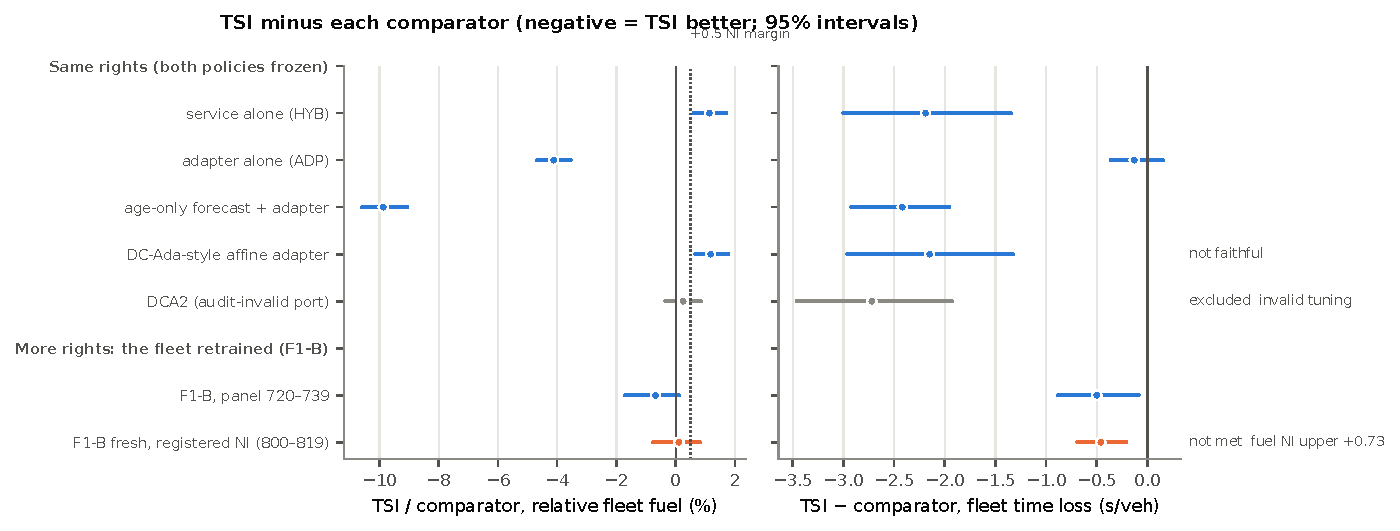
\includegraphics[width=\linewidth]{figs_two_pop/p6_comparators.pdf}
\caption{TSI minus each comparator (negative = TSI better; 95\% intervals). Dotted: the registered $+0.5$ percentage-point
non-inferiority margin for the retrained fleet (W8-2, pending).}\label{fig:comparators}\end{figure}

\subsection{M4: a second network}\label{sec:m4}
Spider network (own-built, \texttt{netgenerate}): a learned all-green light beats the static programs by 57\,s/veh city time loss (two light seeds, development
traffic, C-76); the rule fleet saves $9.2\%$ fuel against $\sigma^*$ (development traffic, C-77), with agent / human time-loss non-inferiority not established on fresh traffic
(upper $+0.55$ / $+0.52$ against the $+0.5$ margin, C-81);
the four-parameter search fleet (R9) failed its pilot gate against the rule there (fuel $+0.40\%$ $[+0.25,+0.53]$ on development
traffic, C-80); the M2 loss and harm replicate with the rule fleet (C-81); fixed-window commitment is again worse than the
no-SPaT fallback, with a different decomposition (no fleet contribution detected, C-82). The retrained-fleet check was not run there, because its registered condition (F1-A1 confirmed; M4-A7) failed (C-85). The
earlier RESCO cologne8 attempt failed at the light baseline and is kept as a negative (C-35, C-36).
\paragraph{TSI on the second network (C-123, C-124).} The same procedure (the forecaster generalized to two or three greens, the adapter
in front of the multi-green learned light's current / next-green inputs, per-light calibration on new tuning traffic) was tested in two registered
confirmation attempts on fresh spider traffic with the rule fleet; with two light seeds, both are conditional on these two lights. The service alone is strongly harmful there (attempt 1: $+20.7\%$ fuel, $+59.5$\,s/veh agent time, with about one
teleport per run; attempt 2: $+19.8\%$, $+57.8$); adding the adapter reduces that harm (TSI $-$ service: $-58.1$ / $-56.4$\,s/veh agent time), but the full configuration failed both attempts. Attempt 1: fuel $-1.66\%$
$[-1.99,-1.38]$, and both city time loss ($+0.55$, upper $+0.91$) and agent time loss ($+1.33$, upper $+1.94$) fail; $0.025$ teleports per
run (R: 0). Attempt 2, with a wider adapter grid at $\alpha=0.025$: fuel $-0.31\%$ $[-0.81,+0.16]$ (no fuel reduction shown); city $+1.32$,
agent $+1.43$ and human $+1.20$\,s/veh all fail. Spider changes the network, the phase structure, the light learner and the receiver at
once, so the failure is not attributed to any one of them. The reduction of harm is relative to a very harmful service; it is not a
deployable result.
\paragraph{Third and last spider attempt (W6-6).} Registered after attempts 1--2 failed, it published SPaT only where the timing is
determined (a yellow whose next green serves the link) and nothing elsewhere. Every published answer was checked against the realized
phase trace, with 0 mismatches. The per-light choices were $(0,0)$ and $(1,0.5)$. It failed at $\alpha=0.0125$: fuel $+0.70\%$
$[+0.41,+1.03]$, agent time $+0.91$\,s/veh. On this network the determined cells alone give the rule fleet no fuel benefit.

\section{Discussion: what the evidence supports}\label{sec:discussion}
\paragraph{Supported.}
\begin{itemize}\setlength\itemsep{0pt}
\item On grid4, with frozen learned signals and fleets, TSI recovered a fuel benefit of about 3.7--3.9\% against the no-SPaT fallback within
the registered time-loss limits. This held in the registered second attempt and again on a third fresh traffic panel.
\item Each half alone failed the joint objective: the service alone costs the agents time; the adapter alone saves no fuel.
\item Scope tests with the design frozen met the limits under higher demand, for a rule and a search-fitted fleet, and at a 75\% fleet
share. At a 25\% share the bound sits at the margin.
\end{itemize}
\paragraph{Not supported.}
\begin{itemize}\setlength\itemsep{0pt}
\item \emph{Equality with retraining on fuel.} On both panels where TSI and the retrained fleet F1-B share cells, no fuel difference was
detected ($-0.68\%$ $[-1.70,+0.11]$ and $-0.60\%$ $[-1.57,+0.19]$). An interval that contains 0 is not an equivalence test, so TSI is not
shown to match retraining on fuel. TSI's city and human time losses were lower on both panels.
\item \emph{A win over a published method.} No published method was reproduced under the same rights and budget. The DC-Ada-style
comparator is not faithful enough to support a claim about DC-Ada. The reports support a method that is useful and meets the registered limits where several
internal comparators do not (the service alone, the adapter alone, the age-only forecast, the light-side commitments and gates, the
DC-Ada-style adapter). The retrained fleet and its Lagrangian variant also met the limits on the third panel. This is not a
state-of-the-art result.
\end{itemize}
\paragraph{Main weaknesses.}
\begin{itemize}\setlength\itemsep{0pt}
\item \emph{External validity.} The method failed all three registered attempts on the second network. One learned-signal family was
tested per network.
\item \emph{Comparator strength.} The published-method comparison is weak, for the reason above.
\item \emph{Checkpoint reuse.} The second attempt and the third panel reuse the first attempt's light and fleet checkpoints, so the
replications are over traffic, not over independently trained policies.
\end{itemize}

\section{Limitations}\label{sec:limits}
\begin{itemize}\setlength\itemsep{1pt}
\item \emph{Simulation only:} SUMO 1.27.1 with its default emission model.
\item \emph{One network.} The method is confirmed on one network (grid4). On the second network (spider: multi-green signals, rule fleet)
the full configuration failed all three registered attempts (C-123, C-124, C-129).
\item \emph{Checkpoint reuse.} The confirmations reuse the same five light and four fleet checkpoints. The family-wise bound over the
first two attempts is 0.075, and the third panel is a fresh-traffic replication only. The crossed bootstrap rests on five light and four
fleet checkpoints, and bounds near a margin are sensitive to the bootstrap draws (25\% share, C-128).
\item \emph{Comparators.} No published method was reproduced under the same rights and budget; the DC-Ada-style comparator differs from
the published algorithm (Section~\ref{sec:w6}). Against the repository's retraining recipe, fuel equivalence is not shown, and on the
third panel the retrained fleet also met the limits.
\item \emph{Deployment cost.} Calibration needs 52 simulated episodes of each deployed signal with a development fleet, so a deployment
needs a site simulator; the transfer of this calibration from a simulator to a real site is untested. The adapter needs per-lane speed
sensing at the signal.
\item \emph{One signal family per network.} grid4 uses a keep-or-switch DQN on halting counts. A signal trained on other inputs may not
shift the same way, and the learned-to-learned swap tested one similar family only.
\item \emph{Forecast details.} The provider of M2b and of the first retrained-fleet attempt leaves a 1\,s early yellow branch (C-84;
corrected in the provider c2 used by F1-B and TSI). The hybrid is exact only for the green after a yellow (C-113). Per-decision analyses are
limited by the simulator's chaotic divergence (C-98).
\item \emph{Provenance.} The provenance of the TSI-chain rows rests on file times and current hashes, not on launch-time records (C-128).
\end{itemize}

\section{Reproducibility}\label{sec:repro}
Registered endpoints come from registered report scripts over saved per-episode rows; every other number comes from the same saved rows
through the analysis named in its ledger row, and the post-hoc ones are labelled (C-55, C-101, C-117, C-125, C-126, C-128).
Provenance gap: the TSI, TSI-2, SHIFT, GEN and spider protocols have no launch-time hash record, and the TSI / HYB rows do not carry the
forecaster, fleet or table hashes (the evaluator's metadata is not written when it is imported; C-128). Every recorded component hash equals
the current source, and every module and input on these paths predates its first use (file times); the freeze record of C-128 lists them. Main files (repository paths):
\begin{itemize}\setlength\itemsep{0pt}
\item protocols: \path{research/city_sim/PROTOCOL_CITY_TSI2_20261005.md} (method and confirmation) and the TSI, SHIFT, GEN, PERF and
SPIDER\_TSI protocols of the same date in the same directory;
\item evaluators: \path{scripts/CITY_eval_n4.py} (grid4 service and \path{--light-obs q:A:B}), run through
\path{scripts/CITY_f1a1_run.py} (loads the light checkpoints t4--t8) and, for fleet shares, \path{scripts/CITY_rho_run.py}; \path{scripts/CITY_m4s_tsi_eval.py} (spider);
\item forecasters: \path{scripts/CITY_n2_fit.py}, \path{scripts/CITY_n2k.py}; calibration: \path{scripts/CITY_tsi2_tune.py};
\item reports: \path{scripts/CITY_tsi2_report.py}, \path{CITY_shift_report.py}, \path{CITY_gen_report.py}, \path{CITY_perf_report.py},
\path{CITY_sptsi_report.py}; figures: \path{scripts/CITY_fig_tsi.py}.
\item wave 6: \path{research/city_sim/PROTOCOL_CITY_WAVE6_20261005.md} (with its pre-run amendment); \path{scripts/CITY_w6_dca_tune.py},
\path{CITY_m4s_tsi3_eval.py}, \path{CITY_w6_m2l.py}, \path{CITY_fleet_train_h45.py}, \path{CITY_lcd.py}, \path{CITY_eval_n9.py}; reports
\path{CITY_w6_report.py} (job 051) and \path{CITY_w6_report_v2.py}; freeze record \path{research/city_sim/FREEZE_RECORD_TSI_20261005.md}.
\end{itemize}
Determinism: \path{PYTHONHASHSEED=0}, \path{OMP_NUM_THREADS=1}. Parity checks KN2 / KT-1 / KS-1 compare offline and online features and
predictions (0 mismatches).

\begin{thebibliography}{99}\small\setlength\itemsep{1pt}
\bibitem{alqithami2026} S.~Alqithami. DC-Ada: Reward-only decentralized sensor adaptation for heterogeneous multi-robot teams. \emph{IEEE Access}, 2026. doi:10.1109/ACCESS.2026.3687163; arXiv:2604.03905.
\bibitem{asadi2011} B.~Asadi, A.~Vahidi. Predictive cruise control: Utilizing upcoming traffic signal information for improving fuel economy and reducing trip time. \emph{IEEE Trans. Control Syst. Technol.} 19(3):707--714, 2011.
\bibitem{ault2021} J.~Ault, G.~Sharon. Reinforcement learning benchmarks for traffic signal control. \emph{NeurIPS Datasets and Benchmarks Track}, 2021.
\bibitem{bansal2019} G.~Bansal, B.~Nushi, E.~Kamar, D.~S.~Weld, W.~S.~Lasecki, E.~Horvitz. Updates in human-AI teams: Understanding and addressing the performance/compatibility tradeoff. \emph{Proc. AAAI}, 2019.
\bibitem{bodenheimer2014} R.~Bodenheimer, A.~Brauer, D.~Eckhoff, R.~German. Enabling GLOSA for adaptive traffic lights. \emph{IEEE Vehicular Networking Conference (VNC)}, 167--174, 2014.
\bibitem{bottom2000} J.~A.~Bottom. \emph{Consistent Anticipatory Route Guidance}. PhD thesis, Massachusetts Institute of Technology, 2000.
\bibitem{dashkovskiy2007} S.~Dashkovskiy, B.~S.~R\"uffer, F.~R.~Wirth. An ISS small gain theorem for general networks. \emph{Math. Control Signals Systems} 19(2):93--122, 2007.
\bibitem{drusvyatskiy2023} D.~Drusvyatskiy, L.~Xiao. Stochastic optimization with decision-dependent distributions. \emph{Math. Oper. Res.} 48(2):954--998, 2023.
\bibitem{eteifa2025} S.~Eteifa, A.~Shafik, H.~Eldardiry, H.~A.~Rakha. Deep learning ensemble approach for predicting expected and confidence levels of signal phase and timing information at actuated traffic signals. \emph{Sensors} 25:1664, 2025. doi:10.3390/s25061664.
\bibitem{genser2024} A.~Genser, M.~A.~Makridis, K.~Yang, L.~Amb\"uhl, M.~Menendez, A.~Kouvelas. Time-to-green predictions for fully-actuated signal control systems with supervised learning. \emph{IEEE Trans. Intell. Transp. Syst.}, doi:10.1109/TITS.2023.3348634; arXiv:2208.11344.
\bibitem{gu2025} H.~Gu, Y.~Zhang, C.~Wang, R.~Jiang, Z.~Qiao, P.~Fan, D.~Jia. A hierarchical deep reinforcement learning framework for traffic signal control with predictable cycle planning. arXiv:2509.03118, 2025.
\bibitem{guo2023} J.~Guo, L.~Cheng, S.~Wang. CoTV: Cooperative control for traffic light signals and connected autonomous vehicles using deep reinforcement learning. \emph{IEEE Trans. Intell. Transp. Syst.} 24(10), 2023. arXiv:2201.13143.
\bibitem{hu2020} H.~Hu, A.~Lerer, A.~Peysakhovich, J.~Foerster. ``Other-play'' for zero-shot coordination. \emph{Proc. ICML}, PMLR 119:4399--4410, 2020.
\bibitem{huang2026} Z.~Huang, Y.~Liu, C.~Liang, G.~Zheng. Planning under observation mismatch for traffic signal control via adaptive modular world models. \emph{ICAPS}, 2026. arXiv:2501.02548.
\bibitem{jiang1994} Z.-P.~Jiang, A.~R.~Teel, L.~Praly. Small-gain theorem for ISS systems and applications. \emph{Math. Control Signals Systems} 7(2):95--120, 1994.
\bibitem{katsaros2011} K.~Katsaros, R.~Kernchen, M.~Dianati, D.~Rieck. Performance study of a Green Light Optimized Speed Advisory (GLOSA) application using an integrated cooperative ITS simulation platform. \emph{IWCMC}, 918--923, 2011. doi:10.1109/IWCMC.2011.5982524.
\bibitem{lopez2018} P.~A.~Lopez, M.~Behrisch, L.~Bieker-Walz, J.~Erdmann, Y.-P.~Fl\"otter\"od, R.~Hilbrich, L.~L\"ucken, J.~Rummel, P.~Wagner, E.~Wie{\ss}ner. Microscopic traffic simulation using SUMO. \emph{IEEE ITSC}, 2018. doi:10.1109/ITSC.2018.8569938.
\bibitem{narang2023} A.~Narang, E.~Faulkner, D.~Drusvyatskiy, M.~Fazel, L.~J.~Ratliff. Multiplayer performative prediction: Learning in decision-dependent games. \emph{J. Mach. Learn. Res.} 24(202):1--56, 2023.
\bibitem{perdomo2020} J.~Perdomo, T.~Zrnic, C.~Mendler-D\"unner, M.~Hardt. Performative prediction. \emph{Proc. ICML}, PMLR 119:7599--7609, 2020.
\bibitem{stone2010} P.~Stone, G.~A.~Kaminka, S.~Kraus, J.~S.~Rosenschein. Ad hoc autonomous agent teams: Collaboration without pre-coordination. \emph{Proc. AAAI}, 2010.
\bibitem{varaiya2013} P.~Varaiya. Max pressure control of a network of signalized intersections. \emph{Transportation Research Part C}, 2013.
\bibitem{wei2018} H.~Wei, G.~Zheng, H.~Yao, Z.~Li. IntelliLight: A reinforcement learning approach for intelligent traffic light control. \emph{Proc. KDD}, 2018.
\bibitem{wei2019} H.~Wei, C.~Chen, G.~Zheng, K.~Wu, V.~Gayah, K.~Xu, Z.~Li. PressLight: Learning max pressure control to coordinate traffic signals in arterial network. \emph{Proc. KDD}, 2019.
\bibitem{zhang2026} Z.~Zhang, C.~Wan, P.~Hao, K.~Boriboonsomsin, M.~J.~Barth, Y.~Liu, S.~Ucar, G.~Wu. HONEST-CAV: Hierarchical optimization of network signals and trajectories for connected and automated vehicles with multi-agent reinforcement learning. arXiv:2602.18740, 2026.
\end{thebibliography}

\appendix
\section{History of the M1 and M2 recipes}
\paragraph{Earlier fleet recipes (C-21 \dots C-37).} No earlier recipe was confirmed (C-21 \dots C-31, corrected C-37); one development checkpoint (R5h\_t0)
passed on fresh traffic; the non-learned $\sigma$-family is a strong baseline ($\sigma=0.3$: $-2.5$ s/veh, $-2.2\%$ fuel).
\paragraph{Fleet diagnostics (C-39 \dots C-43).} D1: the ported phase reward (B) prefers physically better behaviour for large
differences but does not encode the time-loss constraints (it ranks an infeasible fuel-for-time policy far above always-SUMO); PPO from
scratch did not reach always-SUMO even on its training traffic. D2: a hand-written in-class controller (GLOSA target, no release) gives
$-6.7\%$ fuel at equal agent time but harms human cars; a behaviour clone of the heuristic GLOSA trades fuel for time in closed loop.
An evaluation bug (exit release missing in deterministic evaluation) was found by an identity check and fixed (C-41).
A residual on the in-class controller with a crawl-proof group cost (v9) failed its pilot gate; its confirmation was not evaluated (C-47).
Derivative-free policy search over a three-parameter GLOSA family on the deployment objective (fuel with time-loss penalties) returned
the untuned heuristic itself for the pilot search seed; the heuristic fails the $\sigma^*$ comparison on agent time loss (+1.8\,s/veh,
SELECT) and the human-time-loss margin on the width of its 5-seed bound (C-43).
\paragraph{Earlier compatibility probes (C-14 \dots C-34).} Weak learned fleets regressed under light upgrades and a car-side reaction repair
helped (C-14, C-16); non-learned fleet upgrades ($\sigma$, ACC) were not harmed by three learned-light families (C-30, C-32 \dots C-34).

\section{Candidates that failed, and errors found and fixed}
\paragraph{Failed candidates (all reported in the ledger).} M3-E reward-shaped lights (DEV); fixed-window, ETA and receiver-triggered
commitments (WC5, RPC confirmed worse than the fallback, C-86; RPC $2\times2$ diagnostic C-95); per-decision commitment selection (no
selection rule better than a random option out of sample, every interval includes 0; C-96, C-98); tail-support abstention (C-97);
confidence / horizon gates and gate + adapter (C-104, C-105); a CEM-tuned
committed-duration controller (C-116); TSI variants (direct-only hybrid, no SPaT on permissive lefts; C-119); TSI first confirmation
(C-114); spider attempts 1 and 2 (C-123, C-124).
\paragraph{Errors found and fixed.} Found after results that used them, and disclosed with those results: the SPaT timing convention
($+1$\,s, C-71; M2b used the earlier provider) and a yellow branch left 1\,s early by the first correction (C-84, found by an audit;
corrected in the provider c2 for all later runs). Found by self-checks or job failures before the verdict they affected: an xargs job-merging bug (C-92); an exactness error in the committed-duration controller's SPaT (two fixes, KN8-1, C-112);
missing output directories (C-112); a tuple error in the spider provider, caught by KS-2 (C-123 Amendment A1). One provider file was edited
while a job imported it, with no change to the registered code paths (C-103).
Reporting errors corrected in the text: ``exact in yellow'' had been claimed from the 0.1-quantile table (C-113); the spider attempt-2
report header prints attempt 1's traffic range (C-124); the scope report's limits line skipped teleports (C-126); the demand-shift report tested neither teleports nor unfinished trips (both 0
in its 600 runs, C-128); the spider attempt-2 amendment states it was registered before attempt 1's result was read, which the file
times cannot verify (attempt 1's per-seed log lines were printed before the attempt-2 job list was written; C-128).
\section{Validation and pitfalls (QA)}
Reward traces, sentinel readings, residual ratchet, horizon semantics, dominance labels (C-17, C-22, C-25, C-27, C-37, C-38).

\end{document}
